\section{Introduction}
Determining appropriate charges (like \emph{fraud}, \emph{larceny}, and \emph{homicide}) of a case is helpful for legal assistance systems when the user would like to query the system by describing the case, and it is \orange{even more important} when the user has no idea of the legal basis of a case, where the only input he (or she) can give is the fact description of the case. 
% In this situation, predicting appropiate charges would help us to provide the user with relevant  
For example, if the user wants to find similar cases, one can use the predicted charges of the query case to filter out irrelevant results. And if the user wants to know the possible penalties \orange{regarding a case}, one also need to decide appropriate charges first.


In these situations, we need to predict appropirate charges based solely on the fact descriptions of a case. 
However, this charge prediction task is not easy:
(1) The differences between two charges can sometimes be subtle. For example, in the context of criminal cases in China, 
distinguishing \emph{intentional homicide} from \emph{intentional injury} would require determining whether the defendant is intended to kill the victim in the cases where the victim is dead.
% distinguishing \emph{intentional homicide} from \emph{negligent homicide} would require detailed analysis of the behavior of the defendant.
% and \emph{acceptance of bribes} differs from \emph{acceptance of bribes by a non-state functionary} in the occupation of the defendant. 
(2) Multiple crimes may be involved in a single case, which means we need to conduct charge prediction in the multi-label classification paradigm. 
(3)  Although we can expect the model to implicitly learn the legal basis of the judgement through massive training data, the predicted charges are still not convincing enough if no law articles are involved in the prediction. This problem is prominent in countries using civil law system, e.g., China (except Hong Kong), where the judgement is made only based on statutory laws. 
For example, as shown in Figure \ref{fig_example_case}, a judgement document in China always includes relevant law articles (usually in the court view part) to support the decision.  
Even in countries using common law system, e.g., the United States (except Louisiana), where the judgement is based mainly on decisions of previous cases, there are still some statutory laws that need to be followed when making decisions. 

% Therefore, to solve this problem, we need a multi-label classification model, that can effectively capture the overall \orange{framework} along with important details of the fact description, and is able to extract and utilize relevant law articles to build the bridge from the fact description to appropriate charges as well. 

Previous works on charge prediction either use k-Nearest Neighbor (KNN)~\cite{LIU2004case,liu2006exploring} as classifier or need to manually design key factors of specific charges \cite{lin2012exploiting}, thus do not scale well with regard to data size and number of charges. Furthermore, none of them consider the situation where multiple charges are involved. On the other hand, \cite{liu2005classifying,liu2006exploring} also try to find the specific law articles that has been violated, but converts the multi-label problem into multi-class classification by only considering a fixed set of article combinations, therefore does not scale to the situation when a larger set of articles are involved. \cite{liu2015predicting} aims to find relevant articles in a scalable way by doing predilinary classification first and rerank the results afterwards. Although the framework is promising, only shallow, i.e., word-level, semantic features are employed in their work. Furthermore, all of these works treat charge prediction and article prediction separately, ignoring the fact that they can actually benefit each other. 


% Since the judgement of a case often involves deciding appropriate charges, our work is part of the thread of work that tries to predicting the results of a case. Previous works on this thread mainly focuses on a binary classification paradigm. The target is either to decide whether the outcome will side with the plaintiff or defendant~\cite{aletras2016predicting}, or will the justice or the present court affirm or reverse the decision of a lower court~\cite{lauderdale2014scaling,sim2015utility,katz2016general}. Except for their binary prediction nature, these methods either do not use fact descriptions or just capture shallow semantic meaning of the facts, e.g., using Bag-of-Words (BOW). Furthermore, although \cite{aletras2016predicting} also tries to use relevant law articles for prediction, the articles they use are gold standard ones while we extract the relevant article by ourselves.
% Therefore, these methods are not suitable for our task. 

% \footnote{\cite{katz2016general} also use an additional \emph{other} class to represent other complex outcomes.}

% To make conprehensive understanding of the fact description, \orange{we propose to use the framework of the Hierarchical Attention Network (HAN)} \cite{yang2016hierarchical} for document embedding. Specifically, we use a sentence-level and a document-level Gated Recurrent Unit (GRU) to embed each word and each sentence along with their contexts. 
In our proposed method, however, we jointly model the charge prediction and relevant article extraction in a sinble framework, which enables them to influence each other \orange{in a positive way}.
Specifically, to understand the \orange{whole framework} of the facts, inspired by previous works on document classification \cite{tang2015document,yang2016hierarchical}, we use a sentence-level and a document-level Gated Recurrent Unit (GRU) to model the associations among words and sentences.
To capture the important details, we use attention mechanism to select the most informative words or sentences for sentence and document embedding respectively. 
To handle the multi-label nature of the problem, we convert the multi-label target to label distribution, and then use cross entropy as loss function. 
% We find this method works well in our experiments and significantly outperforms the baseline BOW method.
To find relevant law articles in the statutory laws, which contain a large number of articles, to support our charge prediction, we first use a simple BOW-based article classifier to quickly \orange{filter out most of the irrelevant articles}. Then we attentively aggregate the retained top $k$ articles for further charge classification.
% Although the top $k$ articles are noisy, the experimental results show that our attentive aggregation module can further attend to relevant ones and thus improve the prediction performance. 

We evaluate our method by predicting charges in Chinese criminal cases. 
Since the public judgement documents often contain the fact descriptions, relevant law articles and corresponding charges (see Figure \ref{fig_example_case}), they actually provide natural large-scale high-quality trianing data for our task. 
We therefore use rules and regular expressions to extract these information and build a dataset accordingly. The experimental results on this dataset show that our method significantly outperforms the baselie BOW-based Suport Vecotr Machine (SVM) method, and the automatically extracted relevant law articles can clearly improve the model with only facts as input. We also find that our model can effectively attend to the true relevant articles, which to some extent provides us with the legal basis for our charge prediction. Furthermore, since there exists differences between the words used by laymen and legal practitioners, we also annotate 100 news to test the performance of our model on fact descriptions wrtitten by odinary people, which is more useful in practice. The experimental results show that, although trained on judgement document data, our model still has reasonable generalizatoin ability in this situation.

% In this paper, we focus specifically on predicting the charges of criminal cases in China, \orange{which began to} officially publish the judgement documents on China Judgements Online\footnote{http://wenshu.court.gov.cn/} since 2013. Although these judgement documents are unstructured, we can use rules and regular expressions to extract the facts description, relevant law articles, and final charges of the case. This naturally provides us with a high-quality large-scale training dataset for our task.

The contributions of this paper are threefold: 
(1) It proposes a novel neural network model that can jointly utilize the facts and the automatically extracted relevant law articles of a case to predict appropriate charges.
(2) The proposed model can aslo provide legal basis for the charge prediction in the form of weighted relevant law articles.
(2) By further evaluating the model on human labeled news data, it shows that the model trained on judgement documents have reasonable generalization ability on the text written by people who are not legal practitioners.


\begin{figure*}[t!]
\begin{center}
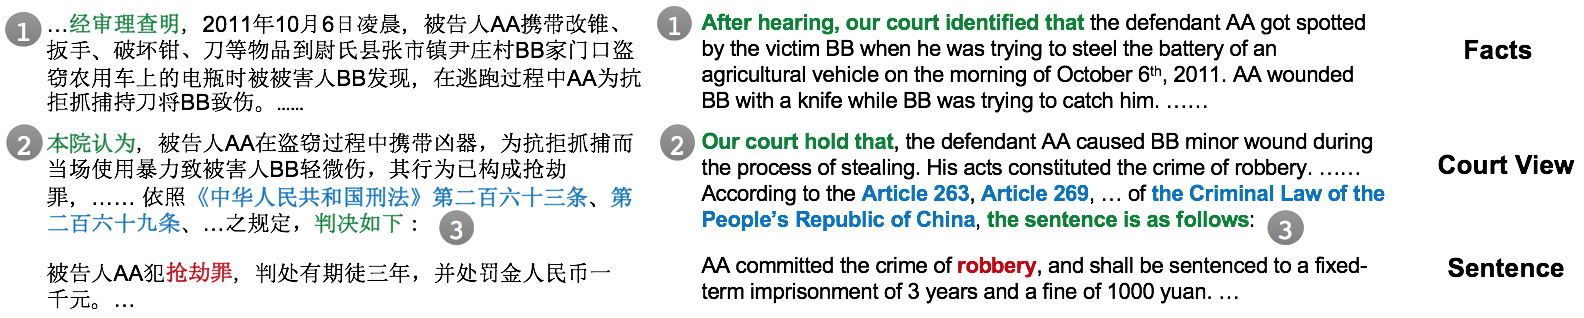
\includegraphics[width=0.97\textwidth]{figures/case.png}	
\caption{Example judgement document excerpt of a Chinese criminal case. Names are anonymized as AA and BB.}
\label{fig_example_case}
\end{center}
\end{figure*}
